\pdfoutput=1
\documentclass[preview]{standalone}

\usepackage[utf8]{inputenc}
\usepackage{lmodern}
\usepackage[T1]{fontenc}

\usepackage{verbatim}
\usepackage{graphicx}
	\DeclareGraphicsRule{*}{mps}{*}{}
\usepackage{xcolor}

\usepackage{tikz}
	\usetikzlibrary{calc}
	\usetikzlibrary{arrows}
	\usetikzlibrary{backgrounds}
	\usetikzlibrary{decorations.pathmorphing}
	\usetikzlibrary{shapes.geometric}
	\tikzset{>=latex'}

\usepackage{amsmath}
\usepackage{amssymb}
\usepackage{dsfont}
\usepackage{nicefrac}
\usepackage{mathrsfs}
\usepackage[Euler]{upgreek}
\usepackage[nointegrals]{wasysym}
\usepackage{booktabs}
\usepackage{float}

\begin{document}

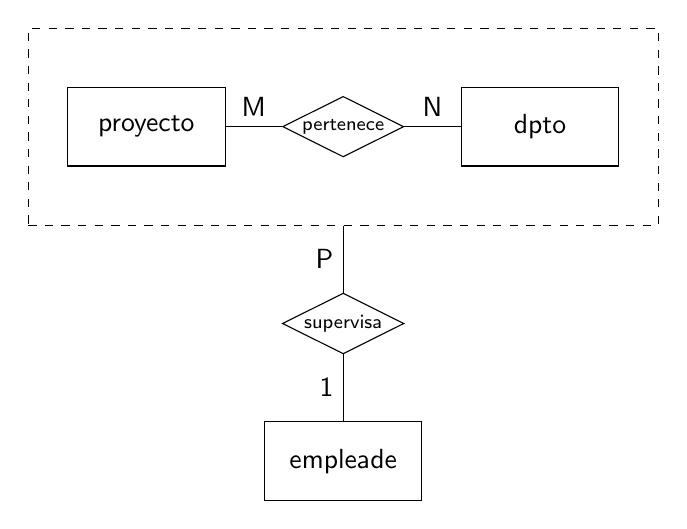
\begin{tikzpicture}[font=\sffamily]
	\node[draw,minimum width=2.0cm,minimum height=1.0cm] (ent1) at (-2.5,0) {proyecto};
	\node[draw,minimum width=2.0cm,minimum height=1.0cm] (ent2) at (2.5,0) {dpto};
	\node[draw,minimum width=2.0cm,minimum height=1.0cm] (ent3) at (0,-4.25) {empleade};
	\node[draw,dashed,minimum width=8.0cm,minimum height=2.5cm] (agregacion) at (0,0) {};
	\node[draw,shape aspect=2,diamond,inner sep=0.2mm] (rel1) at (0,0) {\scriptsize pertenece};
	\node[draw,shape aspect=2,diamond,inner sep=0.2mm] (rel2) at (0,-2.5) {\scriptsize supervisa};
	\draw (ent1) -- node[above]{M} (rel1) -- node[above]{N} (ent2);
	\draw (agregacion) -- node[left]{P} (rel2) -- node[left]{1} (ent3);
\end{tikzpicture}

\end{document}
